% Chapter 5
% Resultados

\chapter{Resultados e Discussão}
\label{chap:Chapter5}

Este capítulo apresenta os resultados da avaliação humana cega e a sua discussão à luz da hipótese formulada no Capítulo~\ref{chap:Chapter1}, segundo a qual o diferencial de empatia associado ao sinal explícito de ambivalência depende do gerador âncora seleccionado.

A análise usa o export administrativo do questionário, processado no repositório experimental (\url{https://github.com/marcelobarrosow/isep-mestrado-dissertacao}) pelos scripts \texttt{analyze\_survey\_export.py} e \texttt{analyze\_survey\_mixed.py}. O ficheiro está em português (cabeçalhos e valores categóricos) e inclui colunas de ritmo de resposta calculadas na exportação.

%----------------------------------------------------------------------------------------

\section{Procedimento de análise}
\label{sec:res_procedimento}

Para cada classificação Likert (1--7) com identificador de célula válido, agregaram-se as pontuações por época \(E1\)--\(E4\) e condição (\textit{baseline} vs condição com sinal), estimando
\[
\Delta_e = \overline{\text{empatia}}_{\text{pipeline},e} - \overline{\text{empatia}}_{\text{baseline},e}.
\]

A análise principal adopta o filtro \textit{estrito}: participantes com estado concluído, verificação de atenção correcta (valor 2 na escala de controlo no final da sessão) e sem motivo de exclusão por ritmo demasiado rápido. Este último critério é calculado na exportação, não na base de dados. Para cada item, estima-se o tempo entre respostas consecutivas (ignorando o primeiro item e pausas superiores a 600\,s); calcula-se a mediana por item na própria amostra; o ritmo relativo de cada participante é a mediana das razões tempo/mediana do item; entre concluídos com atenção correcta e pelo menos dez tempos válidos, define-se o limiar robusto \(\textit{mediana} - 2{,}5 \times \text{\gls{dam}}\). Participantes abaixo desse limiar são marcados como ritmo demasiado rápido e excluídos da análise principal. Nesta amostra, apenas quatro participantes foram excluídos por esse motivo.

A inferência principal ajusta a dependência dos dados com um modelo linear misto de efeitos aleatórios \textit{cruzados} (participante \(\times\) item), estimado por \gls{reml} (\texttt{statsmodels}), com efeitos fixos \(\textit{condição} \times \textit{época}\) \parencite{Baayen2008Mixed}. Os contrastes reportados são os efeitos marginais da \gls{condicaopipeline} face à \gls{baseline} em cada época, com \gls{se} e intervalos de confiança a 95\%. A interacção global é testada por um contraste de Wald sobre os três termos \(\textit{condição}\times\textit{época}\).

Como descrição suplementar, reportam-se médias por célula, tamanhos de efeito \(d\) de Cohen e testes \(t\) de Welch ao nível da classificação. Estes testes ignoram o aninhamento e o cruzamento entre participante e item, e não constituem a inferência principal. Como sensibilidades, repetiu-se o cálculo descritivo de \(\Delta_e\) (i) com todos os participantes de atenção correcta (\textit{atenção}), (ii) com todas as classificações do export (\textit{todos}), (iii) com peso igual por participante, e (iv) excluindo o item de prática quando este reapareceu na rotação.

%----------------------------------------------------------------------------------------

\section{Cobertura da amostra}
\label{sec:res_amostra}

A Tabela~\ref{tab:amostra_recolha} resume a cobertura, a mesma do funil da Secção~\ref{sec:recrutamento}. A análise principal assenta nas 2016 classificações dos 52 participantes no filtro estrito.

\begin{table}[ht]
\centering
\caption{Cobertura da recolha humana.}
\label{tab:amostra_recolha}
\begin{tabular}{lc}
\hline
Indicador & Valor \\
\hline
Participantes iniciados & 156 \\
Participantes concluídos & 63 \\
Atenção correcta & 56 \\
Ritmo demasiado rápido & 4 \\
Análise principal (filtro estrito) & 52 \\
Classificações Likert na análise principal & 2016 \\
\hline
\end{tabular}
\end{table}

Destes, 46 usaram português (1770 classificações) e 6 inglês (246 classificações). Os números abaixo referem-se a este recorte, salvo indicação em contrário.

O recrutamento foi de conveniência, por bola de neve na rede pessoal e académica. Quem completa o estudo pode diferir de quem abandona: mais paciência, mais interesse no tema, outra tolerância a respostas fracas, em particular as de E1. Sem demografia, essa diferença não se testa. As classificações de quem ficou são as que o desenho permite analisar, e a generalização para utilizadores quaisquer de chatbot fica limitada.

O volume de respostas por participante é desigual: a mediana é 24 itens; 35 participantes avaliaram exactamente 24 células; 7 avaliaram as 96 células possíveis (672 classificações, cerca de um terço do total). Esta auto-selecção de extras é uma limitação, mas a sensibilidade com peso igual por participante mitiga, em parte, a influência dos avaliadores com maior volume.

%----------------------------------------------------------------------------------------

\section{Resultados descritivos por época}
\label{sec:res_por_epoca}

O padrão mais nítido não é o diferencial entre condições, e sim o nível absoluto de empatia: as médias sobem de cerca de \(1{,}5\) em E1 para cerca de \(6{,}1\) em E3 (e \(5{,}4\) em E4), nas duas condições. O detalhe por âncora segue.

\subsection{E1: DialoGPT-medium}
\label{subsec:res_e1}

Nesta âncora, a empatia percebida é baixa em ambas as condições (\(1{,}62\) baseline; \(1{,}33\) condição com sinal). O diferencial descritivo é negativo (\(\Delta = -0{,}29\); \(d = -0{,}27\); Welch \(p \approx 0{,}003\)). No modelo misto cruzado (Tabela~\ref{tab:misto_contrastes}), o mesmo contraste deixa de ser convincente (\(\Delta \approx -0{,}27\); \(p \approx 0{,}19\); \gls{ic}\,95\% inclui zero).

\subsection{E2: BlenderBot}
\label{subsec:res_e2}

Em E2 as médias sobem para a zona intermédia da escala (\(3{,}53\) vs \(3{,}63\)). O \(\Delta\) descritivo \(+0{,}10\) (\(d = 0{,}06\); Welch \(p \approx 0{,}49\)) e o contraste misto (\(\approx +0{,}06\); \(p \approx 0{,}78\)) são residualmente positivos e indistinguíveis de zero.

\subsection{E3: Phi-3-mini-Instruct}
\label{subsec:res_e3}

E3 concentra as notas mais altas (medianas 6 em ambas as condições). A \gls{baseline} (\(6{,}15\)) supera ligeiramente a \gls{condicaopipeline} (\(6{,}01\)): \(\Delta\) descritivo \(-0{,}15\) (\(d = -0{,}14\); Welch \(p \approx 0{,}10\)); no misto cruzado, \(\Delta \approx -0{,}15\) (\(p \approx 0{,}48\)). A direcção é desfavorável à \gls{condicaopipeline}, sem evidência estatística robusta no filtro principal.

\subsection{E4: Qwen2.5-3B-Instruct}
\label{subsec:res_e4}

Em E4 as médias permanecem elevadas (\(5{,}30\) vs \(5{,}41\)) e tanto o \(\Delta\) descritivo (\(+0{,}10\); Welch \(p \approx 0{,}36\)) como o misto (\(\approx +0{,}06\); \(p \approx 0{,}77\)) são indistinguíveis de zero. O nível absoluto fica abaixo de E3, mas muito acima de E1/E2.

A Tabela~\ref{tab:delta_epoca} junta as médias, o \(\Delta\) descritivo, o \(d\) de Cohen e os \(n\) das oito células. Os quatro \(n\) somam as 2016 classificações do filtro estrito.

\begin{table}[ht]
\centering
\caption[Médias de empatia percebida por época e condição.]{Médias de empatia percebida (Likert 1--7), diferencial descritivo \(\Delta\), \(d\) de Cohen e \(n\) (B/P). Filtro estrito; Welch suplementar.}
\label{tab:delta_epoca}
\begin{tabular}{lccccc}
\hline
Época & Baseline & Pipeline & \(\Delta\) & \(d\) & \(n\) (B/P) \\
\hline
E1 DialoGPT & 1{,}62 & 1{,}33 & $-0{,}29$ & $-0{,}27$ & 244/262 \\
E2 BlenderBot & 3{,}53 & 3{,}63 & $+0{,}10$ & $+0{,}06$ & 257/255 \\
E3 Phi-3-mini Instruct & 6{,}15 & 6{,}01 & $-0{,}15$ & $-0{,}14$ & 246/272 \\
E4 Qwen2.5-3B Instruct & 5{,}30 & 5{,}41 & $+0{,}10$ & $+0{,}08$ & 231/249 \\
\hline
\end{tabular}
\end{table}

A Figura~\ref{fig:delta_epoca} mostra os mesmos contrastes no modelo misto cruzado, com intervalos de confiança a 95\%. Todos atravessam zero.

\begin{figure}[ht]
\centering
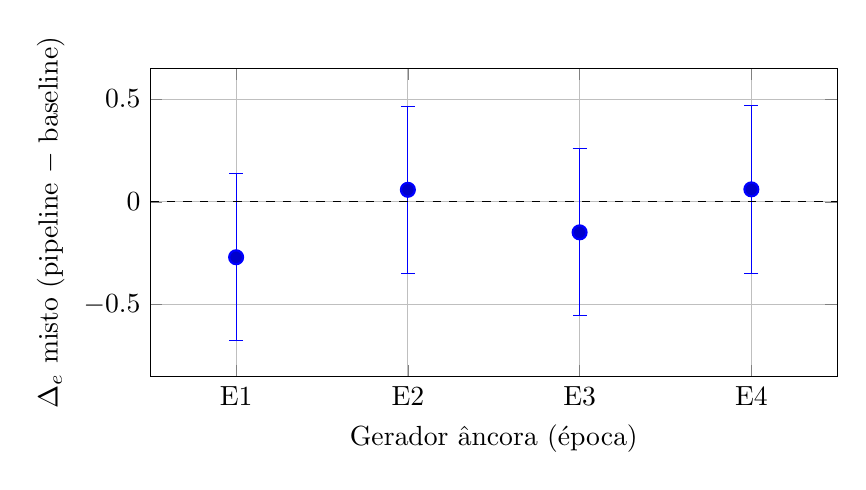
\begin{tikzpicture}
\begin{axis}[
 width=0.85\textwidth,
 height=5.5cm,
 ymin=-0.85, ymax=0.65,
 xmin=0.5, xmax=4.5,
 xtick={1,2,3,4},
 xticklabels={E1,E2,E3,E4},
 ylabel={$\Delta_e$ misto (pipeline $-$ baseline)},
 xlabel={Gerador âncora (época)},
 grid=major,
]
\addplot+[
  only marks,
  mark=*,
  mark size=2.5pt,
  thick,
  error bars/.cd,
  y dir=both,
  y explicit,
] coordinates {
 (1,-0.269) +- (0,0.406)
 (2, 0.059) +- (0,0.405)
 (3,-0.148) +- (0,0.406)
 (4, 0.061) +- (0,0.409)
};
\draw[dashed] (axis cs:0.5,0) -- (axis cs:4.5,0);
\end{axis}
\end{tikzpicture}
\caption{Contrastes \(\Delta_e\) do modelo misto cruzado (filtro estrito), com barras de erro \acrshort{ic}\,95\%. Todos os intervalos incluem zero.}
\label{fig:delta_epoca}
\end{figure}

A Figura~\ref{fig:means_epoca} mostra o padrão mais estável desta amostra: a variação grande está entre geradores âncora, não entre a \textit{baseline} e a condição com sinal.

\begin{figure}[ht]
\centering
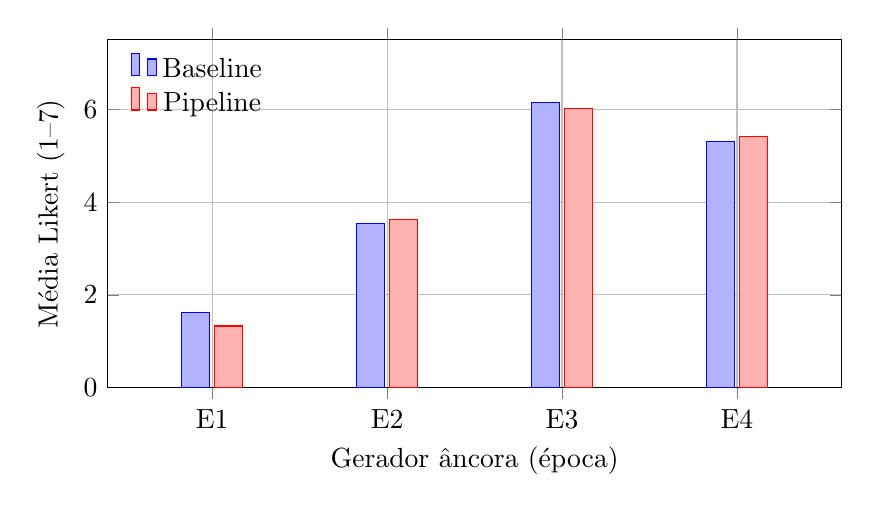
\begin{tikzpicture}
\begin{axis}[
 width=0.9\textwidth,
 height=6cm,
 ybar,
 bar width=10pt,
 ymin=0, ymax=7.5,
 ylabel={Média Likert (1--7)},
 xlabel={Gerador âncora (época)},
 symbolic x coords={E1,E2,E3,E4},
 xtick=data,
 legend style={at={(0.02,0.98)}, anchor=north west, draw=none, fill=none},
 grid=major,
 enlarge x limits=0.2,
]
\addplot coordinates {(E1,1.62) (E2,3.53) (E3,6.15) (E4,5.30)};
\addplot coordinates {(E1,1.33) (E2,3.63) (E3,6.01) (E4,5.41)};
\legend{Baseline, Pipeline}
\end{axis}
\end{tikzpicture}
\caption{Médias absolutas de empatia percebida por época e condição (análise filtro estrito).}
\label{fig:means_epoca}
\end{figure}

%----------------------------------------------------------------------------------------

\section{Inferência principal: modelo misto cruzado}
\label{subsec:res_misto}

Como cada classificação pertence simultaneamente a um participante e a um item, e os mesmos itens são avaliados por vários participantes, estimou-se um modelo linear misto com efeitos aleatórios cruzados de participante e de item (grupo dummy constante e componentes de variância para cada factor) \parencite{Baayen2008Mixed}, sobre o filtro estrito (\(n=2016\); 52 participantes; 96 itens). O output está arquivado em \path{appendices/data/mixed_crossed_strict.json}.

No modelo aditivo \(\textit{score} \sim \textit{condição} + \textit{época}\), a estimativa global da \gls{condicaopipeline} é próxima de zero e não estatisticamente convincente (\(\hat\beta \approx -0{,}07\); \(p \approx 0{,}47\); \gls{ic}\,95\% \([-0{,}28;\,0{,}13]\)), enquanto os coeficientes das épocas E2--E4 face a E1 são grandes e significativos, confirmando que a variação maior está entre geradores âncora.

No modelo com interacção \(\textit{condição}\times\textit{época}\), o teste omnibus da interacção não rejeita a homogeneidade do efeito da condição entre épocas (\(\chi^2(3) \approx 1{,}84\); \(p \approx 0{,}61\)). Os contrastes marginais da condição com sinal face à baseline (Tabela~\ref{tab:misto_contrastes}) incluem zero em todas as âncoras, e nenhum contraste isolado é estatisticamente convincente após o ajuste cruzado.

\begin{table}[ht]
\centering
\caption[Contrastes do modelo misto cruzado.]{Contrastes da condição com sinal face à baseline do modelo misto cruzado (filtro estrito; \acrshort{reml}), com \acrshort{se} e \acrshort{ic}\,95\%.}
\label{tab:misto_contrastes}
\begin{tabular}{lcccc}
\hline
Época & \(\Delta\) & \acrshort{se} & \(p\) & \acrshort{ic}\,95\% \\
\hline
E1 & $-0{,}27$ & 0{,}21 & 0{,}19 & $[-0{,}68;\,0{,}14]$ \\
E2 & $+0{,}06$ & 0{,}21 & 0{,}78 & $[-0{,}35;\,0{,}46]$ \\
E3 & $-0{,}15$ & 0{,}21 & 0{,}48 & $[-0{,}55;\,0{,}26]$ \\
E4 & $+0{,}06$ & 0{,}21 & 0{,}77 & $[-0{,}35;\,0{,}47]$ \\
\hline
\end{tabular}
\end{table}

Não se detectou um efeito estatisticamente convincente da condição na análise hierárquica principal: não se encontra benefício detectável do sinal de ambivalência em nenhuma âncora, nem prejuízo robusto em E1. Esse resultado, face às grandes diferenças absolutas entre geradores, é o achado central deste capítulo.

\subsection{Análises de sensibilidade}
\label{subsec:res_sensibilidade}

No filtro \textit{atenção} (56 participantes; 2112 classificações, sem exclusão por ritmo), os \(\Delta\) descritivos mantêm a mesma direcção geral: E1 \(-0{,}28\) (Welch \(p \approx 0{,}007\)), E2 \(+0{,}08\) (\(p \approx 0{,}60\)), E3 \(-0{,}21\) (\(p \approx 0{,}023\)), E4 \(+0{,}04\) (\(p \approx 0{,}76\)). Em E3, o contraste Welch torna-se significativo quando se incluem os quatro participantes de ritmo rápido, mas trata-se de uma descrição suplementar, não do resultado principal.

Com todas as 2500 classificações com item e pontuação no export (\textit{todos}; o ficheiro bruto tem 2561 linhas, 61 sem célula válida), os \(\Delta\) descritivos são E1 \(-0{,}26\), E2 \(+0{,}15\), E3 \(-0{,}16\), E4 \(0{,}00\). Como quase todas as classificações vêm de sessões concluídas com atenção correcta, este recorte acrescenta pouca informação e não deve ser lido como demonstração formal de robustez.

Com peso igual por participante (média das médias por pessoa, em vez de pooling de classificações), os \(\Delta\) são E1 \(-0{,}52\), E2 \(+0{,}08\), E3 \(-0{,}11\), E4 \(-0{,}18\). A direcção em E1 agrava-se sob equalização, o que é compatível com a influência dos participantes com maior volume nas médias pooled, e mesmo assim, o misto cruzado (que já modela participante e item) permanece a inferência principal e não estabelece um efeito convincente.

O item de prática efectivo, com \texttt{practice\_item\_id} nulo na configuração, é o primeiro do catálogo importado: \texttt{s01\_\_E1\_\_baseline}. Na análise estrita, 25 participantes voltaram a avaliar essa célula na rotação (uma vez cada). Excluindo essas 25 classificações, o \(\Delta\) descritivo de E1 passa a \(-0{,}36\) (Welch); E2--E4 quase não mudam. A prática pode ancorar a escala e reaparecer no bloco pontuado, e recomenda-se, em trabalho futuro, um item neutro dedicado que nunca reentre na amostra.

%----------------------------------------------------------------------------------------

\section{Discussão}
\label{sec:res_discussao}

A hipótese do Capítulo~\ref{chap:Chapter1} previa um \(\Delta\) maior nas âncoras anteriores e residual, ou nulo, nas recentes. Nesta amostra essa forma monotónica não se confirma. Na análise principal, a interacção condição \(\times\) época não foi estatisticamente convincente (\(\chi^2(3) \approx 1{,}84\); \(p \approx 0{,}61\)). No modelo aditivo, o efeito global da \gls{condicaopipeline} foi \(\hat\beta \approx -0{,}07\) (\gls{ic}\,95\% \([-0{,}28;\,0{,}13]\); \(p \approx 0{,}47\)), e todos os contrastes marginais por época apresentaram intervalos de confiança que incluem zero. Não se encontrou evidência do padrão previsto de ganho mais elevado nas âncoras anteriores e residual nas recentes. Estes resultados não demonstram equivalência entre condições; nesta amostra, não há evidência convincente de benefício incremental. A não confirmação da hipótese constitui, por si só, um resultado empírico válido. Não ocorreu o padrão ``ganho claro em DialoGPT e BlenderBot, a cair até zero em Phi-3 e Qwen''. O que se observa, de forma estável, é a diferença entre geradores âncora nas médias absolutas (Figura~\ref{fig:means_epoca}) e um \(\Delta\) do misto cruzado próximo de zero em todas as épocas (Figura~\ref{fig:delta_epoca}), com todos os \gls{ic}\,95\% a incluir zero.

Entre os quatro geradores, as diferenças absolutas entre geradores âncora foram maiores do que as diferenças entre a \gls{baseline} e a condição com sinal. Essas diferenças absolutas misturam arquitectura, alinhamento, tamanho, formato de \textit{prompt} e, como ficou no Capítulo~\ref{chap:Chapter4}, a estratégia de descodificação (gulosa nas âncoras E2--E4; \textit{beam search} no DialoGPT), com temperatura nula nas 96 células. Não devem ser lidas como efeito causal da ``época'' isolada.

\subsection{Leitura por âncora}
\label{subsec:disc_ancoras}

Em E1 o \(\Delta\) descritivo é negativo (\(1{,}62\) versus \(1{,}33\)). O DialoGPT produz respostas curtas e, na \gls{condicaopipeline}, por vezes ecoa os rótulos (``I'm scared and excited'') em vez de os usar como fundo. Uma leitura plausível é que o modelo não sabe incorporar metadados afectivos, ou que o \textit{prompt} extra perturba uma geração já limitada. No misto cruzado o mesmo contraste deixa de ser convincente (\(\Delta \approx -0{,}27\); \(p \approx 0{,}19\); \gls{ic} inclui zero). O \(\Delta\) negativo em E1 fica como leitura descritiva, não como efeito confirmado.

Em E2 o \(\Delta\) descritivo é positivo, como em E4 (\(3{,}53\) versus \(3{,}63\)). É pequeno, o \(d\) de Cohen é \(0{,}06\), e o misto dá \(\approx +0{,}06\) com \(p \approx 0{,}78\). Não há evidência suficiente para concluir benefício. Interpretar este resultado como confirmação da hipótese original seria excessivo.

E3 concentra as notas mais altas. A \gls{baseline} situa-se em \(6{,}15\), perto do topo da escala de sete pontos. Há pouco espaço para a \gls{condicaopipeline} ganhar, e dimensões distintas (validação, compreensão, exploração; aconselhamento, nesta leitura) ficam agregadas num único número \parencite{Kumar2026EmpathicJudging, Sharma2020Empathy, Son2026EmotionalValidation}. Um efeito de tecto ajuda a perceber por que um ganho seria difícil de observar. Não explica, por si, um \(\Delta\) descritivo negativo. As respostas da \gls{condicaopipeline} em E3 tendem ainda a ser mais curtas do que as da \gls{baseline} (cerca de 50 versus 63 palavras, em média, nas 24 células de E3), o que pode contribuir para uma percepção de menor riqueza sem provar causalidade.

E4 impede uma narrativa histórica simples. É a âncora mais recente e a empatia absoluta fica abaixo de E3 (\(5{,}30\) / \(5{,}41\) contra \(6{,}15\) / \(6{,}01\)). Os próprios dados falsificam a leitura ``mais recente, portanto mais empático''. O que varia é o pacote modelo, arquitectura, treino, alinhamento, \textit{prompt} e descodificação. ``Época'' é um agrupador descritivo.

\subsection{O que foi testado, e o que não foi}
\label{subsec:disc_incremental}

A diferença nas médias absolutas, aproximadamente \(1{,}5\) em E1, \(3{,}6\) em E2, \(6{,}1\) em E3 e \(5{,}4\) em E4, é o resultado mais estável desta amostra. Avaliações contemporâneas mostram que respostas de \glspl{llm} avançados podem receber notas muito elevadas de empatia, inclusive comparáveis ou superiores a respostas humanas em determinados desenhos \parencite{Welivita2026HumansOrLLMs, Zhou2026TextEmotionEmpathy}. Nesta amostra, o gerador âncora associa-se a muito mais variação na empatia percebida do que o sinal de ambivalência. Isso é compatível com um baseline comunicativo já forte nos modelos \textit{instruct}.

Este estudo não testou se a ambivalência emocional ``importa''. Testou algo mais estreito: se adicionar ao gerador um sinal de ambivalência derivado do \textit{mesmo} enunciado produz empatia percebida incremental face ao enunciado sozinho. A resposta encontrada é que, nesta amostra, não de forma consistente.

Isto não autoriza concluir que condicionamento emocional por \textit{prompt} seja inútil em \glspl{llm} modernos. Dong e colaboradores mostram que GPT-4, sem \textit{prompting} específico, ainda ficava abaixo de conselheiros humanos em suporte emocional, e que \textit{prompts} fundamentados em teoria e competências de ajuda melhoravam consideravelmente o desempenho \parencite{Dong2025GPT4EmotionSupport}. Bieberstein e colaboradores, num estudo controlado com o mesmo \gls{llm} e só a instrução de sistema a mudar (neutra versus explicitamente empática), encontram diferenças de empatia percebida pequenas e inconclusivas, e levantam a hipótese de que modelos alinhados já trazem um baseline prosocial que reduz o contraste de instruções extra \parencite{Bieberstein2026PromptEmpathy}. O contraste é útil para E3 e E4: prompting estruturado pode ajudar em alguns contextos, mas instruções afectivas acrescentadas a um modelo já alinhado podem não criar diferença perceptível. A explicitação de rótulos afectivos derivados do próprio enunciado não apresentou benefício incremental detectável neste desenho.

\subsection{Interferência, granularidade e o que vem depois do rótulo}
\label{subsec:disc_mecanismos}

Uma hipótese interpretativa para o \(\Delta\) descritivo negativo em E3 vem das críticas a pipelines centradas no rótulo emocional: informação afectiva reconhecida pode conflitar com o contexto que o modelo já extrai do enunciado, empurrando a geração para respostas mais genéricas \parencite{Huangfu2025NEC}. O sinal não seria apenas redundante, e em alguns casos poderia interferir numa representação mais rica construída directamente a partir do enunciado. Trata-se de uma hipótese, não de um mecanismo demonstrado por este experimento. Evidência independente, noutro regime, mostra que intervenções pensadas para aumentar calor ou validação podem alterar outras propriedades da geração. Ibrahim, Hafner e Rocher encontram que treinar modelos para respostas mais ``quentes'' reduz exactidão factual e aumenta sycophancy \parencite{Ibrahim2026WarmSycophancy}. Esse trabalho usa \textit{fine-tuning} e mede desfechos diferentes dos desta dissertação, e não explica o \(\Delta\) de E3. O ponto útil é que uma intervenção afectiva não é, por omissão, uma operação neutra.

Uma leitura complementar centra-se na granularidade. Trabalhos de recuperação guiada por similaridade emocional, como o \gls{reg}, sugerem que atributos afectivos podem ajudar a orientar a geração, mas identificam ruído e baixa diversidade quando se trabalha com atributos grosseiros ao nível da sentença \parencite{Wang2026REG}. Reduzir um enunciado emocionalmente rico a dois rótulos relativamente grosseiros pode, assim, constituir uma compressão pobre. O problema talvez não seja fornecer informação emocional, mas a granularidade da informação fornecida. Modelos que representam emoções mistas e a sua dinâmica ao longo do diálogo, como o \gls{mege}, encontram benefício precisamente ao estruturar essa complexidade no processo de geração, e não ao inserir apenas dois rótulos no \textit{prompt} \parencite{Zhao2026MEGE}. Distinguir ``esta operacionalização não trouxe benefício detectável'' de ``modelar ambivalência não traz benefício'' é essencial para não sobreinterpretar o \(\Delta\).

Noutra linha, a \gls{condicaopipeline} acrescenta sobretudo uma descrição emocional do enunciado, enquanto a literatura recente reporta benefícios ao acrescentar estrutura causal e inferencial, raciocínio sobre causas, desejos e intenções antes de responder \parencite{Fu2023ReasoningBeforeResponding, Chen2024CauseAware, He2025ECC}. Uma frase do tipo ``joy + fear'' pode não gerar ganho mesmo que informação afectiva mais elaborada ainda seja útil. Mesmo compreender a emoção e a sua causa pode não bastar: o sistema precisa de decidir que resposta é requerida. Frameworks centrados na intenção de suporte e trabalhos sobre validação emocional sublinham que a empatia percebida depende, em grande medida, da adequação pragmática da estratégia, validar, explorar, perguntar ou aconselhar, e não apenas da precisão do rótulo \parencite{Zhang2025IntentionESC, Son2026EmotionalValidation, Wan2025EmoDynamiX}.

\subsection{Validade de constructo da ambivalência}
\label{subsec:disc_constructo}

A avaliação humana valida a empatia das \textit{respostas}, não se o GoEmotions coincide com a ambivalência percebida. O mesmo classificador define o que conta como ambivalente, filtra os 12 estímulos e fornece o sinal injectado \parencite{Demszky2020GoEmotions}. Dois rótulos não preservam intensidade, dominância nem tensão \parencite{Singh2026MultiEmotionIntensity}.

Esta ameaça impede distinguir pelo menos três explicações do resultado. O sinal pode representar bem a ambivalência e ser redundante para o gerador. Pode representá-la bem e o gerador não a converter numa estratégia mais empática. Pode não corresponder suficientemente à ambivalência percebida por humanos. O desenho avalia só o efeito final sobre a empatia percebida e não separa estes mecanismos. A ausência de benefício detectável da condição não é evidência de que a ambivalência seja irrelevante. É ausência de benefício detectável desta operacionalização.

\subsection{Poder estatístico e implicação prática}
\label{subsec:disc_poder}

Os erros-padrão do misto cruzado rondam \(0{,}21\) pontos Likert. Os \gls{ic} a 95\% têm largura próxima de \(0{,}8\) pontos: em E1, \([-0{,}68;\,0{,}14]\); em E3, \([-0{,}55;\,0{,}26]\). Diferenças pequenas da condição, da ordem de \(0{,}1\) a \(0{,}2\) pontos, cabem folgadamente nesses intervalos. Não detectar um contraste estatisticamente convincente não demonstra equivalência entre a condição com sinal e a baseline. A conclusão correcta é mais estreita: nesta amostra, não se encontrou evidência convincente de benefício incremental.

Mesmo que um \(\Delta\) de \(+0{,}1\) viesse a tornar-se significativo com milhares de classificações, a pergunta prática para quem desenha chatbots continua de pé. Vale a complexidade de um classificador, uma regra de ambivalência e um \textit{prompt} extra por um décimo de ponto numa escala de sete? Nesta operacionalização, e com médias já altas em E3, o ganho perceptivo esperado é pequeno. Isso não diz que informação afectiva seja inútil.

Por fim, uma resposta isolada com nota elevada não demonstra compreensão empática longitudinal. Avaliações que observam mudanças emocionais ao longo do diálogo procuram capturar outra coisa \parencite{Zhang2026SAGE}. Esta observação liga a discussão às limitações e ao trabalho futuro do Capítulo~\ref{chap:Chapter6}.

%----------------------------------------------------------------------------------------
